\chapter{Related Work}
\todo: remake description! \\ %In chapter 2 A1, A3, A4, A6, A7, A10, A14 and 15 are already discussed. In this chapter the remaining aspects are analysed by investigating how other researchers decided on them. The remaining aspects are dependent variables (A2), the task (A5), the MR technology to use (A8), the tracking technology (A9), the behaviour of the instructions (A11), the measures to apply (A12) and the considered body parts (A14). These aspects are better discussed at existing systems to make sure the study having a high validity. This chapter is structured by means of the perspective though the independent variables, namely ego-centric, exo-centric and the combination of both. In this subchapters the aspects are discussed and concluded. In the overall conclusion a decision is made for the aspects by comparing them to each other. eg, the task must be suitable for all perspectives.

\section{Overview}
Here will stand an aggregated overview about work. The systems of the next section are not mentioned here.
\section{Comprehension of the papers analysed}
because I chose to split by topics (task, measures...) here is an overview over the papers that going to be discussed.
\subsection{In detail - A VR Dance Training System Using Motion Capture Technology}
\begin{itemize}
	\item[Hardware:] Optical Motion tracking, 3D screen
	\item[Task:] Dance moves
	\item[Perspectives:] exo-centric
	\item[Measures:] position
	\item[investigation:] Comparing video based learning with VR learning with feedback
	\item[variables:] independent: training method, dependent: precision
	\item[Outcome:] better assists in learning compared to traditional video approach, as well as more motivation an fun
\end{itemize}

\subsection{in detail - Onebody: Remote Posture Guidance System using First Person View in Virtual Environment}
\begin{itemize}
	\item[Hardware:] Kinect, Oculus Rift
	\item[Task:] sports, dance, martial arts, yoga
	\item[Perspectives:] Ego-centric
	\item[Measures:] Position, completion time, subjective score
	\item[investigation:] comparing different remote guidance systems: onebody, pre recorded video, video conference, VR third person
	\item[variables:] Independent: training method, dependent: performance
	\item[Outcome:] Onebody offers better posture accuracy in delivering movement instructions
\end{itemize}

\subsection{In detail - Training for Physical Tasks in Virtual Environments: Tai Chi}
\begin{itemize}
	\item[Hardware:] HMD, Optical motion tracking
	\item[Task:] Tai Chi
	\item[Perspectives:] Ego-centric, exo-centric \& egocentric combined
	\item[Measures:] position
	\item[investigation:] different perspectives on virtual avatar(s)
	\item[variables:] independent: perspectives, dependent: precision
	\item[Outcome:] None representation proved to be significantly better than the other representations
\end{itemize}

\subsection{YouMove: Enhancing Movement Training with an Augmented Reality Mirror}
\begin{itemize}
	\item[Hardware:] Augmented reality mirror, Kinect
	\item[Task:] dance moves, sport moves
	\item[Perspectives:] exo-centric, ego-centric, combined
	\item[Measures:] position matching
	\item[investigation:] Comparing video based learning with YouMove
	\item[variables:] independent: training method, dependent: precision
	\item[Outcome:] learning and short-term retention better than traditional video representation
\end{itemize}

\subsection{Generic Heading}
\begin{itemize}
	\item[Hardware:] 
	\item[Task:] 
	\item[Perspectives:] 
	\item[Measures:] 
	\item[investigation:] 
	\item[variables:] 
	\item[Outcome:] 
\end{itemize}

\subsection{Generic Heading}
\begin{itemize}
	\item[Hardware:] 
	\item[Task:] 
	\item[Perspectives:] 
	\item[Measures:] 
	\item[investigation:] 
	\item[variables:] 
	\item[Outcome:] 
\end{itemize}

\subsection{Generic Heading}
\begin{itemize}
	\item[Hardware:] 
	\item[Task:] 
	\item[Perspectives:] 
	\item[Measures:] 
	\item[investigation:] 
	\item[variables:] 
	\item[Outcome:] 
\end{itemize}

\subsection{Generic Heading}
\begin{itemize}
	\item[Hardware:] 
	\item[Task:] 
	\item[Perspectives:] 
	\item[Measures:] 
	\item[investigation:] 
	\item[variables:] 
	\item[Outcome:] 
\end{itemize}

\subsection{Generic Heading}
\begin{itemize}
	\item[Hardware:] 
	\item[Task:] 
	\item[Perspectives:] 
	\item[Measures:] 
	\item[investigation:] 
	\item[variables:] 
	\item[Outcome:] 
\end{itemize}

\section{Analysis}
\subsection{Study task}
%---
The task in Chua's \cite{Chua} \textbf{Tai Chi trainer} is \--- as the name indicates \--- a Tai Chi motion. A professional Tai Chi trainer was invited to perform a so called \textit{Tai Chi form} and recorded offline. This \textit{form} was segmented in four ca. 20 seconds long sequences (Motion 1-4). "Motion 1 featured simple hand movements and a 90 degree turn to the right; motion 2 had little hand motion, a 180 degree turn of the feet, and some turning of the upper body; motion 3 featured slow hand motions, large movement of the feet, and some turning of the thorax; and motion 4 featured swift hand movement and turning of the thorax and hips but little movement of the feet." \cite{Chua}. Error measurements indicated that all motion but motion 1 had the same difficulty, being significantly easier. This movements can be classified as \textit{sequential movements} according to chapter 2 \todo ref. 40 volunteers conducted the movements in a study to evaluate their system. They randomized the condition (described in next chapter, compare figure \ref{fig:taichiperspectives} condition a-e) and the motion to minimize learning effects. For each motion and condition pair, the Tai Chi student were asked to match the Tai Chi teachers demonstration during twelve repetitions.\\ \\
%---
\textbf{YouMove} by Anderson et al. \cite{Anderson2013} is a movement training system, suitable for a vast range of moves. A movement can be recorded and then edited by an authoring tool. After the editing, the movement is added to the internal library, from which it can be chosen by a student. For the study itself, an author or the paper \--- though no professional \--- recorded four movements. Two of them from ballet and two abstract movement. The authors decided to variate the difficulty of the task, namely "the ballet movements [...] were easier to conceptualise and required only moderate movement.", while "the abstract movements were more difficult to perform, as they were a series of postures with no clear structure and required substantial movement." The movements consisted of four keyframes. Keyframes are important points during the movements, determined and set by the person recording a movement.
%---
%---
%---
%---
%---
%---

\subsubsection{Conclusion}


\subsection{Implemented Perspective}
%---
Chua et al. \cite{chua} implemented five different perspectives to teach Tai Chi, compare \ref{fig:taichiperspectives}. There are three exo-centric perspectives (a-c, further called conditions a-c) and two ego-centric perspectives combined with exocentric (d,e, further called conditions d,e). In \textbf{One on One} the student stand next to one teacher, which is closest to a real world training scenario \ref{fig:taichiperspectives}(a). In con \--- \textbf{Four Teachers} \--- the student is surrounded by four teachers, with the student in the middle \ref{fig:taichiperspectives}(b). The \textbf{Side by Side} \ref{fig:taichiperspectives}(c) condition shows four pairs of teacher and student in the same formation as in condition (b). The first ego-centric \& combined condition is called \textbf{Superimposition 1} \ref{fig:taichiperspectives}(d). Here the formation still remains, but the student in the middle is surrounded by four more students. On each of the student a red wireframe teacher is superimposed. \textbf{Superimposition 2} \ref{fig:taichiperspectives}(e), is similar to Superimposition one and differs only in the visual representation: the student is now a green, transparent wireframe. Chua et al. use no pure ego-centric perspective, since in the latter two conditions the teacher can be seen also from the exo-centric perspective.
\begin{figure}
	\centering
	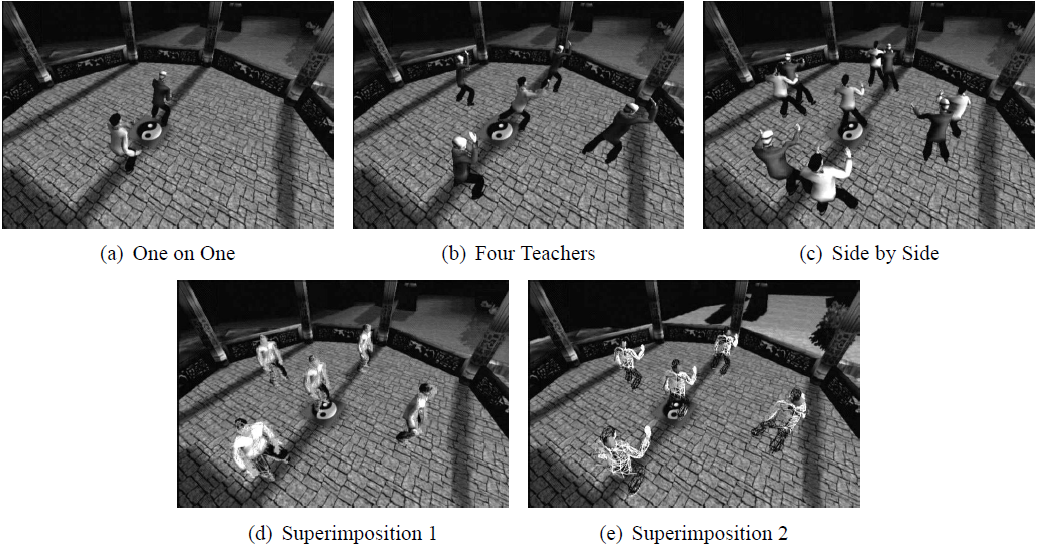
\includegraphics[width=1.0\textwidth]{img/taichi_perspectives.png}
	\caption{Used perspectives at \cite{Chua}}
	\label{fig:taichiperspectives}
\end{figure}\\
%---
YouMove \cite{Anderson2013} provides multiple stages for the learning process: (1) Demonstration, (2) Posture Guide, (3) Movement Guide, (4) Mirror, (5) On your own. In (1) the user sees a video of the movement, though the perspective is exo-centric. In stage 2 \& 3 the user is superimposed by a skeleton, though the perspective changes to ego-centric. Stage 4 \& 5 does not allow a view on the teachers representation. After each stage a feedback is given. This view provides multiple perspectives for the four keyframes: a skeleton of the teacher and student superimposed (ego-centric), a video of the teachers demonstration and a video of the moves of the student (exo-centric) \--- this can be seen as a combination of both perspectives but only in the aftermath of the learning sequence.
%---
%---
%---
%---
%---
%---
\subsubsection{Conclusion}

\subsection{Guidance visualisation}
%--- shape and colour
Chua's \textbf{Tai Chi training} scenario takes place in pure VR using a HMD. The lessons are conducted in a virtual pergola standing in a nature or park environment. In condition a to c (compare \ref{fig:taichiperspectives}), the student and the teacher are rendered as non transparent, high realism degree avatars. However, in condition d and e, the visual appearance changes. In condition (d) the student is still rendered normally but the teacher is now represented as a red wireframe. Condition (e) was introduced late in the development of the system based on early subject feedback. The students here are rendered as green wireframe avatars and the teacher as red wireframe avatars.\\
In terms of guiding technique, the student is presented the pre recorded motion of the teacher. The teacher avatar performs the motion in question and the student tries to mimic this motion. During the mimicking process no feedback is provided to the student. But in condition (d) and (e) the teacher is superimposed on the students avatar. This can be interpreted as feedback since the difference between the students e.g. arm position and the teachers arm position can be seen easily.\\ \\
%---
\textbf{YouMove} uses Microsoft Kinect (\todo ref) to record motions and to track the student. The recorded instruction as well as the students movements are projected on an AR mirror. The special about this mirror is, that the degree of reflection can be changed by simply adjusting the light in the room. With this, the student can see his own real body as reflection as well as the projection of a beamer simultaneously. If the room is bright, the student sees only his reflection and in a dark room only the projection is visible.\\
The visualisation of the teacher itself is rendered in a low degree of realism \--- only a stick figure in yellow. During the feedback screen after each stage, the student is also rendered as a stick figure but in blue.\\
For teaching, YouMove utilise the above mentioned five training stages. In the first stage (Demonstration), a video of the teacher performing the movements is shown. The student only sees the video and not the reflection of the own body. The second stage (Posture guide) a video and the stick figure of the student are shown, but still not the own reflection. The student is asked to match they postures at specific keyframes, where the demonstration stops. After matching the posture of a keyframe, the demonstration moves on to the next keyframe. In the third stage (Movement Guide) the demonstration no longer stops at the keyframes. Furthermore, the reflection and the projection are visible simultaneously, the student is superimposed by the teachers stick figure. (\todo change skeleton to stick figure). Stage four (Mirror) is like the name indicates: the student stands in front of the mirror seeing only his own reflection but additionally audio queues are provided. In the last stage (On you own) even the mirror is removed and the student performs the movements without any guidance.\\
In terms of feedback, Anderson et al. state "[...] the availability and modality of feedback can greatly impact skill acquisition". To match this, feedback is a part of YouMove. During the second stage (Demonstration), red circles indicate misplaced limbs. The bigger the circle the bigger the misplacement. Additionally, a side view on the scene is faded in. At the end of each stage, a so called "summary feedback" is provided. Here the both stick figures of the teacher and student are superimposed and a video of both can be seen. Eventually a score is provided, which will be explained in the next chapter

%---
%---
%---
%---
%---
%\subsection{Visual Appearance}
%\subsection{Degree of Realism}
%\subsection{Guidance Techniques}
%\subsection{Feedback}


\subsubsection{Conclusion}

\subsection{Dependent variables}
%---
In the Tai Chi trainer by Chua et al. \cite{Chua}, the students task is to mimic the motion of a pre recorded teacher. While the independent variables are the above mentioned perspectives (conditions a-e) and the motions, the independent variable is the precision of the performed movements. To measure this precision, twelve bones of the students were tracked, namely: upper and lower arms, hands, upper and lower legs, and feet. The bones are hierarchical structured with a parent and child end. After a normalization of the parents position and bone length, an error was calculated:
\begin{equation}
	\todo
\end{equation}
This error can be seen as the euclidean distance between the teacher's and the student's position of a bone. This error was calculated for every frame of the roughly 20 seconds with a rate of 60 fps:
\begin{equation}
	\todo
\end{equation}
The last four out of twelve trials were considered. So the measure of precision is described as:
\begin{equation}
	\todo
\end{equation}
This measure is an implementation of chapter 2 ref \todo.
Chua et al. found two major faults in this method of precision determination: yaw shift (\todo add in chapter 2 a definition of dofs) and time shift. To overcome the first, the initial position of the student was taken into account, the latter was fixed with a time frame comparison of 120 frames. Eventually this result was normalized with the difficulty (average number of errors per motion) of the motion task. This will be discussed in detail in the Projects Report. In addition, a post questionnaire was conducted where the students were asked to rate the difficulty of the representations. The results are discussed in the next section.\\ \\
%---
While Chua et al. calculate the error of the performed movement over all tracked limbs, Anderson et al. take one single joint with the greatest error and \--- even more constricting \--- only the keyframe joints (important joints, specified by the teacher) are taken into consideration. The dependent variable is a score between 0 and 10. An offset 15 cm results in a score of 7.5 and no error results in a score of 10. The offset is imply the eucledean distance. This error measurement corresponds to chapter 2 \todo. To overcome time shift errors, a window of 0.5 seconds is added. If the teacher specified that timing is important, this window is halved, if precision is set as important, 15cm offset results in a score of 7.5. "This values are determined by experimentation"
%---
%---
%---
%---

\subsubsection{Conclusion}

\subsection{Results}
%---
Chua et al. compare different perspectives (conditions a-e) on the teacher and the student. The independent variables are the above mentioned precision of the students performance. By comparing the results they found condition a (One on One), b (Four Teachers), c (Side by Side) and e (Superimposition 2) aim the same precision. Only e (Superimposition 1) aimed significantly worse than the others. At the same time, the questionnaire indicated that the subjective difficulty of condition d and e (Superimposition 1 and 2) was the highest. "In fact, all of the subjects who tried Superimposition 2 thought it was the most difficult. Interestingly, although subjects considered Superimposition 2 very difficult compared to the other layouts, average error on that layout was not significantly greater than the other non-superimposed layouts." \cite{Chua}. The Authors argue this result as following:
\begin{itemize}
	\item simultaneously watching the teacher and performing own movements could interfere each other.\\
	Chua et al. suggests to choose wisely for the task to suit into VR training.
	\item latency and performance correlates strongly. A lower latency could lead to better performance.\\
	Since Chua et al. \cite{Chua} was developed in 2003, there is a large improvement in latency nowadays.
	\item To reduce latency a low polygon count on the high realism degree avatars was used. More polygons could lead to better performance.\\
	The system was run on a Pentium 3 processor. Today's graphic cards and processors are way above this mark, a higher polygon count is easily achievable.
	\item The field of view was very small.\\
	Today's VR HMDs probably provide a higher field of view (e.g. HTC Vive, 110$^\circ$).
\end{itemize}
%---
Anderson et al. compared YouMove with traditional video training, resulting in the independent variables \textit{YouMove} and \textit{Video}. The study was conducted with eight participants in a two factor repeated-measures design. Each participant had one ballet and one abstract task with both conditions. \textit{YouMove} scored significantly better than \textit{Video} by a factor of 2. \todo: elaborate a little bit more.
%---
%---
%---
\subsubsection{Conclusion}






\section{in detail - Onebody: Remote Posture Guidance System using First Person View in Virtual Environment}
(I tried both: split by topic and by paper. This paper is described in one, not split by the aspects above. I will split that soon.)
Onebody by Hoang et al. \cite{Reinoso2016} is a VR system for remote posture guidance. Onebody is designed for sports or physical activity training like yoga, dance or martial arts. The student and the teacher are both tracked by skeletal tracking. The visualisation of this tracking are shown via a VR headset, allowing the student to follow the instruction of the teacher in first person view of the teacher - which means the student "stands inside the body of the teacher". Both, the student and the teacher are visualised by stick figures. The teachers avatar is red, the students blue and matching joints are green like shown in figure \ref{fig:ob1} left. Figure \ref{fig:ob1} right shows the scene from the first person perspective.
\begin{figure}
	\centering
	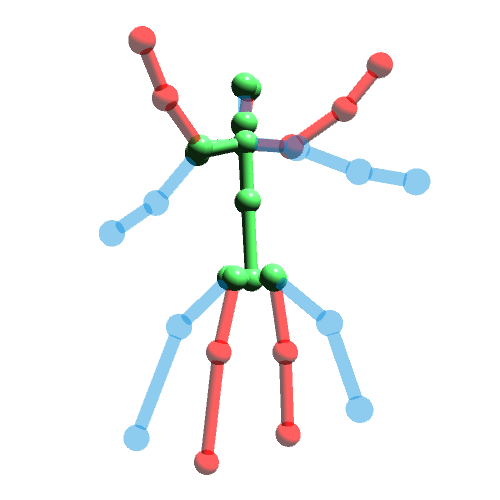
\includegraphics[width=0.225\textwidth]{img/onebody1.png}
	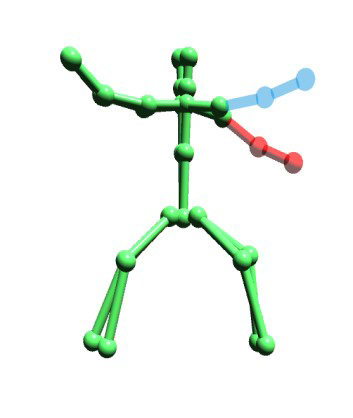
\includegraphics[width=0.225\textwidth]{img/onebody2.png}
	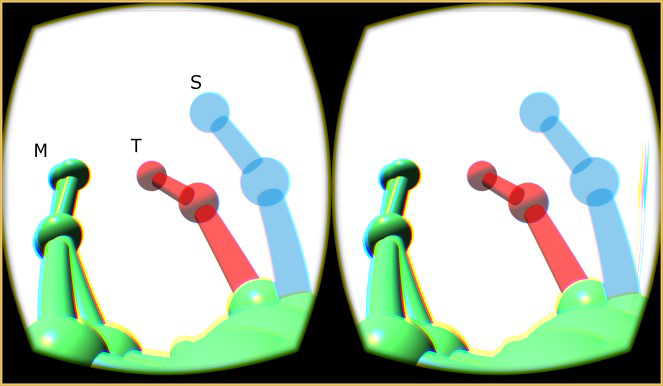
\includegraphics[width=0.45\textwidth]{img/onebody3.png}
	\caption{Left: student avatar (blue) and teacher avatar (red). Green limbs are matching limbs. Right: students view on the scene.\cite{Reinoso2016}}
	\label{fig:ob1}
\end{figure}
When the teacher moves his limbs, the student can see the movement emerging from himself. Now the student can move his own limbs to mimic the movement till the teachers posture is matched. The teacher sees the students limbs likewise allowing him to give instant feedback to the student. Thus, "Onebody provides a medium to deliver body movement instructions for non-collocated instructor and learner." \todo. The visualisations are attached to the hip but keeps the mapping between the user and corresponding avatar. To overcome different body sizes, the avatars are normalised and scaled to the size of the person seeing the avatars.\\
For transfering data, both the teacher and the student are clients in a server-client system. The clients are sending the their tracking data to the server which is broadcasting it to the clients. The comparison of the limbs for colour coding is performed on the client side. The matching of the limbs is calculated by the position of the single limbs (see equation \eqref{eq:constanterror}) with a threshold of 5cm to reduce jitter and tracking errors. Limbs in question are wrist, elbow, shoulder, hip, knee and ankle. The feedback with colour codes is provided in realtime.\\
With this system hoang et al. designed a user study to evaluate the performance of posture accuracy and user's preference. Their main hypotheses is "\textit{Onebody delivers better posture accuracy than existing remote movement instruction methods}". "Posture accuracy is determined by the extend to which the student can replicate the final posture as instructed and demonstrated by the instructor." In addition, completion time and a subjective score of the instructor are considered.
To test the hypothesis, Onebody was compared with three other remote posture training methods (independent variables): pre recorded video, video conference (Skype), VR 3rd person perspective. Each of the systems differs to Onebody in terms of synchronous interaction, VR medium and perspective see figure \ref{fig:ob2}.
\begin{figure}
	\centering
	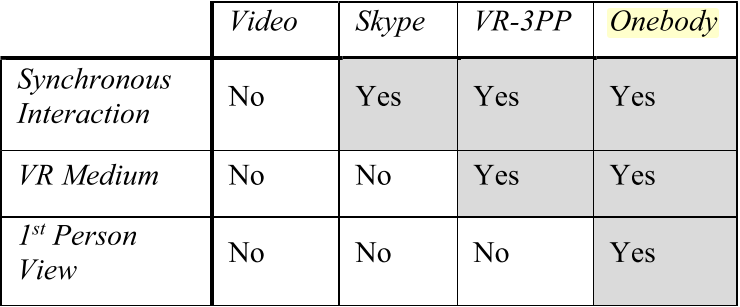
\includegraphics[width=0.5\textwidth]{img/onebody_training_methods.PNG}
	\caption{Training methods and their differences used in the study to evaluate Onebody \cite{Reinoso2016}}
	\label{fig:ob2}
\end{figure}
The study was a 4x4 within subject. Each participant stated with a training session in which the not collocated instructor teach a posture physically and verbally. Verbal feedback was given the training repeated until the student was confident. After that the final posture was recorded. A set of four of postures with every system were performed with different complexities.\\
The results show a significant difference in accuracy. Onebody performed significantly better in over video conference, 3rd person VR and pre recorded video. Furthermore, the completion time was significantly higher with Onebody as in the other three systems. The subjective score of the instructor showed no significant differences. A post questionnaire indicated that Onebody is harder to understand and use than the other systems, but at the same time it also indicated that Onebody was perceived to be more exact. Participants rated video conference as their most preferred system over Onebody and 3rd person VR.

\section{conclusion}
Here will stand an overall conclusion
\begin{table}[H]
	\begin{tabular}{|l|l|l|l|l|l|}
		\hline
		Study Task & Implemented Perspective & Guidance Visualisation & Dependent Variables & Results & \\ \hline
		&  &  &  &  & \\ \hline
	\end{tabular}
	\caption{Table of the conclusion}
\end{table}

\begin{comment}

%----------------------------------------------------
Researchers utilised the theory of the last chapter to design MR Motor Learning systems in various ways. They differ in the technology, tasks, perspectives measures etc. In this chapter we analyse these systems to extract valuable insights to design a MR Motor learning System. First we analyse the aspects of MRML systems. After that we take a close look on some systems how they conducted their investigation and their outcome.

\section{Aspects of MR Motor Learning systems}
paper to come:
\begin{itemize}
	\item Cruz: Cyclone uppercut
	\item Davcev: AR Environment for Dance Learning
	\item Chan: Immersive Performance training Tools Using Motion Capture Technology
	\item Han: AR-Arm: Augmented Visualization for Guiding Arm Movment in the First-Person Perspective
	\item han: My Tai-Chi Coaches: An Augmented-Learning Tool for Practicing Tai-Chi Chuan
\end{itemize}

\subsection{Method}
Jacky Chan et al. \todo created a VR dance training system using an optical motion capturing system to compare the movements performed by the student with movements from the avatar. These movements are presented to the student as a 3D rendering on large screen. The movements of the students are visualised on the same screen as a coloured stick figure. The student mimics these movements and gets instant feedback as well as a feedback as a summary.

In contrast, Onebody by Hoang et al. \todo use a VR headset for a first person remote posture guidance system. 

\subsection{Tasks}
In Chan et al. \todo the dance student is presented a virtual avatar performing dance moves of A-go-go or Hip-Hop style. The avatars movement is based on the motion capturing data of a professional dancer. Onebody \todo is not only restricted to dance moves but also include other posture based sports or physical activities like Yoga or Mixed Martial Arts.

Onebody \todo uses a number of martial arts postures or stances.
\begin{itemize}
	\item Onebody: 16 artificial postures not from but like: tai chi, matial arts
	\item VR Dance Trainer: dance movements, 15 min for each move
	\item you move: various movements to perform. using a whip, baseball, boxing, ballet, dance moves
	\item training archived physical skills IVE: physical skills in sport activities, especially baseball pitching
\end{itemize}

\subsection{Measures and variables}
Jacky Chan et al. \todo defined 19 body parts that are considered in the measure of the performance of the dancing student. They name three features to compare the difference between two motions common: joint position, joint velocity and joint angle. Chan investigated which of these features suits most to judge the two dancing motions. The outcome of this investigation names the joint position to have the highest discriminative power. Hence, the joint position suits them best for their evaluation, Chan et al. calculate a score of the position error for each of the defined body parts, as well as an overall score. 

Onebody \todo uses skeletal of the instructor and the student
"Posture accuracy is determined by the extend to which the student can replicate the final posture as instructed and demonstrated as by the instructor." Independent variable: mothods for posture training. dependent variables: performance factors of posture accuracy, completion time, subjective instructor rating, users preference.

\begin{itemize}
	\item scientific work, how to measure movements: hachimura et al, yoshimura et al, qian et al, kwon et al, all use joint angles,  (mentioned in: vr dance trainer)
	\item onebody: skeletal tracking, how much percent do the postures match? 3d positions of limbs measured: wrist, elbow, shoulder, hip knee ankle. so angle between bones is the main measure for accuracy. additionally a subjective instructor score was recorded. And, completion time, topped by 2 min.
	\item VR Dance trainer: there are 3 common features for measuring hte difference between movements: joint position, velocity, angle. they tested which feature descibes movements best: joint position. base line vs post training movements are compared.
	\item you move: in each keyframe, score based on the joint with the maximum error, measured in euclidean distance. but only "important joints" are measured. timing errors: 0.5s error on each side of the frame for matching posture. is timing important, the window is reduced to 0.25s. max eucl. distance is linear mapped to a score. 0 error is 10 (max), 10cm is 7.5 what is the score to pass. if precision is important, 10cm needed for pass.
\end{itemize}

\subsection{Considered Body Parts}
scientific work, how to measure movements: hachimura et al, yoshimura et al, qian et al, kwon et al, all use joint angles

error prevention \todo

\section{Detailed description of 6-10 papers incl. Table}
%hier werden die paper detailiert vorgestellt von denen ich dann meine tasks, measures, methode und variablen ableite. am ende zusammenfassung in einer tabelle






\section{Research Gap}
lücken in der aktuellen forschung die sich lohnen zu untersuchen. \todo

\subsection{Conclusion of VR motor learning systems}
to conclude we have a look a Table \ref{table:ConclusionVRSystems}
\begin{table}[]
	\begin{tabular}{|l|l|l|l|l|l|}
		\hline
		Name & Hardware & Perspectives & Task & Measures & Variables \\ \hline
		Onebody &  &  &  &  &  \\ \hline
		VR dance trainer &  &  &  &  &  \\ \hline
		&  &  &  &  &  \\ \hline
		&  &  &  &  &  \\ \hline
		&  &  &  &  &  \\ \hline
		&  &  &  &  &  \\ \hline
	\end{tabular}
	\caption{Summary of proposed MR learning systems}
	\label{table:ConclusionVRSystems}
\end{table}


Research questions?\\
Hypothesis?\\
\end{comment}